\documentclass[12pt]{article}
\textwidth=17cm \oddsidemargin=-0.9cm \evensidemargin=-0.9cm
\textheight=23.7cm \topmargin=-1.7cm
\headheight=14.5pt

\usepackage{amssymb, amsmath, amsfonts}
\usepackage{moreverb}
\usepackage{graphicx}
\usepackage{enumerate}
\usepackage{graphics}
\usepackage{color}
\usepackage{array}
\usepackage{float}
\usepackage{hyperref}
\usepackage{textcomp}
\usepackage{alltt}
\usepackage{physics}
\usepackage{nicefrac}
\usepackage{mathtools}
\usepackage{tikz}
\usepackage{pgfplots}
\pgfplotsset{compat=1.13}
\usetikzlibrary{positioning}
\usetikzlibrary{arrows}
\usepackage{bigints}
\usepackage[utf8]{inputenc}
\usepackage[english]{babel}
\usepackage{amsthm}
\usepackage{fancyhdr}
\usepackage[makeroom]{cancel}
\pagestyle{fancy}
\allowdisplaybreaks

\newcommand{\E}{\varepsilon}

\newcommand{\suchthat}{\, \mid \,}
\newcommand{\ol}[1]{\overline{#1}}
\newcommand{\bbar}[1]{\overline{#1}}
\newcommand{\inpd}[1]{{\left< \, #1 \, \right>}}
\renewcommand{\theenumi}{\alph{enumi}}
\newcommand\Wider[2][3em]{%
\makebox[\linewidth][c]{%
  \begin{minipage}{\dimexpr\textwidth+#1\relax}
  \raggedright#2
  \end{minipage}%
  }%
}

\def\R{\mathbb{R}}
\def\C{\mathbb{C}}
\def\H{\mathcal{H}}
\DeclareMathOperator*{\esssup}{\text{ess~sup}}
\newcommand{\resolv}[1]{\rho(#1)}
\newcommand{\spec}[1]{\sigma(#1)}
\newcommand{\iffR}{\noindent \underline{$\Longrightarrow$:} }
\newcommand{\iffL}{\noindent \underline{$\Longleftarrow$:} }
\newcommand{\lightning}{\textbf{\Huge \Lightning}}
\newcommand{\spt}[1]{\text{spt}(#1)}
\def\ran{\text{ ran}}
   
\newenvironment{myprob}[1]
    {%before text commands
    %{\Huge \_ \_ \_ \_ \_ \_ \_ \_ \_ \_ \_ \_ \_ \_ \_ \_ \_ \_ } \\
    \noindent{\Huge$\ulcorner$}\textbf{#1.}\begin{em}
    }
    { 
    %after text commands
    \end{em} \\ \hphantom{l} \hfill {\Huge$\lrcorner$} }
%	{\noindent \rule{7.5cm}{2pt} \textgoth{#1} \rule{8.cm}{2pt} \begin{em}}
%	{\end{em}\\ \vspace{0.1pt}\noindent \rule{\textwidth}{2pt}}
%
\setcounter{section}{-1}




\begin{document}
\lhead{MATH228B}
\chead{Carter Johnson - Homework 04}
\rhead{\today}

{\let\newpage\relax} 


%%%%%%%%%%%%%%%%%%%%%%%%%%%%%%%%%%%%%%%%%%%%%%%%%%%%% P2
\begin{myprob}{Problem 1}
Write programs to solve the advection equation
$$u_t + au_x = 0, $$
on $[0,1]$ with periodic boundary conditions using upwinding and Lax-Wendroff.  For smooth solutions, we expect upwinding to be first-order accurate and Lax-Wendroff to be second-order accurate, but it is not clear what accuracy to expect for nonsmooth solutions.
\end{myprob}
\begin{enumerate}[(a)]
\item Let $a=1$ and solve the problem up to time $t=1$.  Perform a refinement study for both upwinding and Lax-Wendroff with $\Delta t=0.9a\Delta x$ with a smooth initial condition.  Compute the rate of convergence in the 1-norm, 2-norm, and max-norm.  Note that the exact solution at time $t=1$ is the initial condition, and so computing the error is easy.

I used the smooth initial condition $u(x,0) = \sin(\pi x)$ on [0,1].  I started with an initial number of grid points $N_x = 90$ and initial number of time steps $N_t = 100$ so that $$\dfrac{\Delta t}{a\Delta x} = \dfrac{N_x}{N_t} = 0.9.$$

To implement Upwinding on the periodic domain, I used the iteration matrix
$$S = \qty(\begin{array}{cccc} 
1-\nu & & &  \nu \\
\nu & 1-\nu & &  \\
& \ddots & \ddots &  \\
& & \nu & 1-\nu
\end{array}) $$
and followed the scheme $$u^{n+1} = S u^{n}$$ for $N_t$ time steps.

To implement Lax-Wendroff on the periodic domain, I used the iteration matrix
$$LW = \qty(\begin{array}{cccccc} 
1-\nu^2 & \frac{\nu^2-\nu}{2} & & & &  \frac{\nu^2+\nu}{2} \\
\frac{\nu^2+\nu}{2} & 1-\nu^2 & \frac{\nu^2-\nu}{2} & & & \\
& \ddots & \ddots & \ddots & & \\
& & \ddots & \ddots & \ddots &  \\
& & & \frac{\nu^2+\nu}{2} & 1-\nu^2 & \frac{\nu^2-\nu}{2} \\
\frac{\nu^2-\nu}{2} & & & & \frac{\nu^2+\nu}{2} & 1-\nu^2
\end{array}) $$
and followed the scheme $$u^{n+1} = LW u^{n}$$ for $N_t$ time steps.

From there, I performed a refinement study on both upwinding and Lax-Wendroff methods by doubling $N_x$ (and subsequently $N_t$).  The results are tabulated as follows. As we double the number of grid points, we see that for the upwinding method, the error in the 1-norm and 2-norm are reduced by a factor of 2, so upwinding is indeed first-order in the 1-norm and 2-norm.  For the max-norm however, the error is only reduced by a factor of 1.4 ($\approx \sqrt{2}$), so the method is still convergent but less than first-order in the max-norm.

For Lax-Wendroff, we see that doubling the number of grid points reduces the error in the 1-norm and 2-norm by a factor of 4, so the method is indeed second-order in the 1-norm and 2-norm.  For the max-norm, the error is only reduced by a factor of 2.8, so the method is still convergent but somewhere between first and second-order in the max-norm.

% \begin{table}[H]
% \caption{Upwinding Refinement Study - Errors and Runtimes}
% \centering\begin{tabular}{||c|ccc|cc||}
% \hline \hline
%     $N_x$ & $\norm{u(x,0)-u(x,1)}_1$ & $\norm{u(x,0)-u(x,1)}_2$ & $\norm{u(x,0)-u(x,1)}_{\infty}$ &   Runtime &   Runtime Ratios \\
% \hline
%     90 &    0.0138114   &    0.0153396   &      0.0216905   &  0.002116 &          0       \\
%    180 &    0.00694327  &    0.00771191  &      0.0109058   &  0.003697 &          1.74716 \\
%    360 &    0.00348112  &    0.00386653  &      0.00546805  &  0.007303 &          1.97539 \\
%    720 &    0.00174294  &    0.00193592  &      0.00273779  &  0.015256 &          2.089   \\
%   1440 &    0.000872067 &    0.000968623 &      0.00136984  &  0.034589 &          2.26724 \\
%   2880 &    0.000436183 &    0.000484477 &      0.000685154 &  0.074314 &          2.14849 \\
%   5760 &    0.000218129 &    0.00024228  &      0.000342636 &  0.24084  &          3.24084 \\
%  11520 &    0.000109074 &    0.00012115  &      0.000171333 &  0.771567 &          3.20365 \\
%  23040 &    5.45392e-05 &    6.05778e-05 &      8.567e-05   &  2.97792  &          3.85957 \\
%  46080 &    2.72702e-05 &    3.02896e-05 &      4.28359e-05 & 11.749    &          3.94537 \\
% \hline \hline
% \end{tabular}
% \end{table}
\begin{minipage}{0.5\textwidth}
\begin{table}[H]
\caption{Upwinding - 1-Norm Convergence}
\centering\begin{tabular}{||c|cc||}
\hline \hline
    $N_x$ &   $\norm{u(x,0)-u(x,1)}_1$ &   Ratios \\
\hline
    90 &    0.0138114   &  0       \\
   180 &    0.00694327  &  1.98918 \\
   360 &    0.00348112  &  1.99455 \\
   720 &    0.00174294  &  1.99727 \\
  1440 &    0.000872067 &  1.99863 \\
  2880 &    0.000436183 &  1.99932 \\
  5760 &    0.000218129 &  1.99966 \\
 11520 &    0.000109074 &  1.99983 \\
 23040 &    5.45392e-05 &  1.99991 \\
 46080 &    2.72702e-05 &  1.99996 \\
\hline \hline
\end{tabular}
\end{table}
\end{minipage}%
\begin{minipage}{0.5\textwidth}
\begin{table}[H]
\caption{Upwinding - 2-Norm Convergence}
\centering\begin{tabular}{||c|cc||}
\hline \hline
    Nx &   $\norm{u(x,0)-u(x,1)}_2$ &   Ratios \\
\hline
    90 &    0.0153396   &  0       \\
   180 &    0.00771191  &  1.98908 \\
   360 &    0.00386653  &  1.99453 \\
   720 &    0.00193592  &  1.99726 \\
  1440 &    0.000968623 &  1.99863 \\
  2880 &    0.000484477 &  1.99931 \\
  5760 &    0.00024228  &  1.99966 \\
 11520 &    0.00012115  &  1.99983 \\
 23040 &    6.05778e-05 &  1.99991 \\
 46080 &    3.02896e-05 &  1.99996 \\
\hline \hline
\end{tabular}
\end{table}
\end{minipage}
\begin{minipage}{0.5\textwidth}
\begin{table}[H]
\caption{Upwinding - Max-Norm Convergence}
\centering\begin{tabular}{||c|cc||}
\hline \hline
    Nx &   $\norm{u(x,0)-u(x,1)}_\infty$ &   Ratios \\
\hline
    90 &      0.0216905   &  0       \\
   180 &      0.0109058   &  1.40655 \\
   360 &      0.00546805  &  1.41036 \\
   720 &      0.00273779  &  1.41228 \\
  1440 &      0.00136984  &  1.41325 \\
  2880 &      0.000685154 &  1.41373 \\
  5760 &      0.000342636 &  1.41397 \\
 11520 &      0.000171333 &  1.41409 \\
 23040 &      8.567e-05   &  1.41415 \\
 46080 &      4.28359e-05 &  1.41418 \\
\hline \hline
\end{tabular}
\end{table}
\end{minipage}%
\begin{minipage}{0.5\textwidth}
\begin{table}[H]
\caption{Upwinding- Runtimes}
\centering\begin{tabular}{||c|cc||}
\hline \hline
    Nx &   Runtimes &   Runtime Ratios \\
\hline
    90 &   0.002116 &          0       \\
   180 &   0.003697 &          1.74716 \\
   360 &   0.007303 &          1.97539 \\
   720 &   0.015256 &          2.089   \\
  1440 &   0.034589 &          2.26724 \\
  2880 &   0.074314 &          2.14849 \\
  5760 &   0.24084  &          3.24084 \\
 11520 &   0.771567 &          3.20365 \\
 23040 &   2.97792  &          3.85957 \\
 46080 &  11.749    &          3.94537 \\
\hline
\end{tabular}
\end{table}
\end{minipage}
% \begin{table}[H]
% \caption{Lax-Wendroff Refinement Study - Errors and Runtimes}
% \begin{tabular}{||c|ccc|cc||}
% \hline \hline
%     $N_x$ & $\norm{u(x,0)-u(x,1)}_1$ & $\norm{u(x,0)-u(x,1)}_2$ & $\norm{u(x,0)-u(x,1)}_{\infty}$ &   runtime &   runtime ratios \\
% \hline
%     90 &    0.000617121 &    0.000685479 &      0.000969175 &  0.001979 &          0       \\
%    180 &    0.000154332 &    0.000171414 &      0.000242401 &  0.003954 &          1.99798 \\
%    360 &    3.85844e-05 &    4.28562e-05 &      6.06068e-05 &  0.008095 &          2.04729 \\
%    720 &    9.64619e-06 &    1.07142e-05 &      1.51521e-05 &  0.017808 &          2.19988 \\
%   1440 &    2.41155e-06 &    2.67856e-06 &      3.78805e-06 &  0.044824 &          2.51707 \\
%   2880 &    6.02889e-07 &    6.69641e-07 &      9.47015e-07 &  0.106869 &          2.38419 \\
%   5760 &    1.50722e-07 &    1.6741e-07  &      2.36754e-07 &  0.284315 &          2.66041 \\
%  11520 &    3.76805e-08 &    4.18526e-08 &      5.91885e-08 &  0.939381 &          3.30401 \\
%  23040 &    9.42014e-09 &    1.04631e-08 &      1.47971e-08 &  3.94602  &          4.20066 \\
%  46080 &    2.35503e-09 &    2.61579e-09 &      3.69928e-09 & 15.9845   &          4.0508  \\
% \hline \hline
% \end{tabular}
% \end{table}
\begin{minipage}{0.5\textwidth}
\begin{table}[H]
\caption{Lax-Wendroff - 1-Norm Convergence}
\centering\begin{tabular}{||c|cc||}
\hline \hline
    $N_x$ & $\norm{u(x,0)-u(x,1)}_1$ &  Ratios \\
\hline
    90 &    0.000617121 &  0       \\
   180 &    0.000154332 &  3.99867 \\
   360 &    3.85844e-05 &  3.99985 \\
   720 &    9.64619e-06 &  3.99996 \\
  1440 &    2.41155e-06 &  3.99999 \\
  2880 &    6.02889e-07 &  4       \\
  5760 &    1.50722e-07 &  4       \\
 11520 &    3.76805e-08 &  4       \\
 23040 &    9.42014e-09 &  4       \\
 46080 &    2.35503e-09 &  4       \\
\hline \hline
\end{tabular}
\end{table}
\end{minipage}
\begin{minipage}{0.5\textwidth}
\begin{table}[H]
\caption{Lax-Wendroff - 2-Norm Convergence}
\centering\begin{tabular}{||c|cc||}
\hline \hline
$N_x$  & $\norm{u(x,0)-u(x,1)}_2$ &  Ratios \\
\hline
    90 &    0.000685479 &  0       \\
   180 &    0.000171414 &  3.99897 \\
   360 &    4.28562e-05 &  3.99975 \\
   720 &    1.07142e-05 &  3.99994 \\
  1440 &    2.67856e-06 &  3.99998 \\
  2880 &    6.69641e-07 &  4       \\
  5760 &    1.6741e-07  &  4       \\
 11520 &    4.18526e-08 &  4       \\
 23040 &    1.04631e-08 &  4       \\
 46080 &    2.61579e-09 &  4       \\
\hline \hline
\end{tabular}
\end{table}
\end{minipage}
\begin{minipage}{0.5\textwidth}
\begin{table}[H]
\caption{LW - Max-Norm Convergence}
\centering\begin{tabular}{||c|cc||}
\hline \hline
   $N_x$ & $\norm{u(x,0)-u(x,1)}_{\infty}$ &   Ratios \\
\hline
    90 &      0.000969175 &  0       \\
   180 &      0.000242401 &  2.82788 \\
   360 &      6.06068e-05 &  2.8283  \\
   720 &      1.51521e-05 &  2.8284  \\
  1440 &      3.78805e-06 &  2.82842 \\
  2880 &      9.47015e-07 &  2.82843 \\
  5760 &      2.36754e-07 &  2.82843 \\
 11520 &      5.91885e-08 &  2.82843 \\
 23040 &      1.47971e-08 &  2.82843 \\
 46080 &      3.69928e-09 &  2.82843 \\
\hline \hline
\end{tabular}
\end{table}
\end{minipage}
\begin{minipage}{0.5\textwidth}
\begin{table}[H]
\caption{Lax-Wendroff - Runtimes}
\centering\begin{tabular}{||c|cc||}
\hline \hline
    $N_x$ &   Runtimes &   Runtime Ratios \\
\hline
    90 &   0.001979 &          0       \\
   180 &   0.003954 &          1.99798 \\
   360 &   0.008095 &          2.04729 \\
   720 &   0.017808 &          2.19988 \\
  1440 &   0.044824 &          2.51707 \\
  2880 &   0.106869 &          2.38419 \\
  5760 &   0.284315 &          2.66041 \\
 11520 &   0.939381 &          3.30401 \\
 23040 &   3.94602  &          4.20066 \\
 46080 &  15.9845   &          4.0508  \\
\hline\hline
\end{tabular}
\end{table}
\end{minipage}

\item Repeat the previous problem with the discontinuous initial condition
$$u(x,0) = \begin{cases}1 & \text{ if } |x-1/2|<1/4 \\ 0 & \text{ otherwise } \end{cases}.$$
\end{enumerate}

Again, I started with an initial number of grid points $N_x = 90$ and initial number of time steps $N_t = 100$ so that $$\dfrac{\Delta t}{a\Delta x} = \dfrac{N_x}{N_t} = 0.9.$$
From there, I performed a refinement study on both upwinding and Lax-Wendroff methods by doubling $N_x$ (and subsequently $N_t$).  The results are tabulated as follows. As we double the number of grid points, we see that for the upwinding method, the errors in the 1-norm is reduced by a factor of 1.4 and the errors in the 2-norm are reduced by a factor of 1.18, so upwinding is less than first-order in the 1-norm and 2-norm.  For the max-norm however, the errors are actually growing, so it seems that the method is not convergent for discontinuous initial data in the max-norm.

For Lax-Wendroff, we see that doubling the number of grid points reduces the error in the 1-norm by a factor of 1.5 and and in the 2-norm by a factor of 1.24, so the method is less than first-order in the 1-norm and 2-norm.  For the max-norm, the error is growing so the method is not convergent for discontinuous initial data in the max-norm.

\begin{table}[H]
\caption{Upwinding Refinement Study - Errors and Runtimes}
\centering\begin{tabular}{||c|ccc|cc||}
\hline \hline
    $N_x$ & $\norm{u(x,0)-u(x,1)}_1$ & $\norm{u(x,0)-u(x,1)}_2$ & $\norm{u(x,0)-u(x,1)}_{\infty}$ &   Runtime &   Runtime Ratios \\
\hline
    90 &     0.0527461  &      0.123893  &         0.45129  &  0.001942 &          0       \\
   180 &     0.0374545  &      0.104568  &         0.465538 &  0.00373  &          1.9207  \\
   360 &     0.0265402  &      0.0880948 &         0.475626 &  0.007954 &          2.13244 \\
   720 &     0.0187865  &      0.074148  &         0.482763 &  0.014647 &          1.84146 \\
  1440 &     0.0132911  &      0.06238   &         0.487811 &  0.034097 &          2.32792 \\
  2880 &     0.00940068 &      0.0524674 &         0.491381 &  0.096329 &          2.82515 \\
  5760 &     0.00664816 &      0.0441248 &         0.493905 &  0.237519 &          2.46571 \\
 11520 &     0.00470127 &      0.0371066 &         0.49569  &  0.863169 &          3.63411 \\
 23040 &     0.00332441 &      0.0312037 &         0.496953 &  4.11757  &          4.77029 \\
 46080 &     0.00235075 &      0.0262395 &         0.497845 & 19.8843   &          4.82914 \\
\hline \hline
\end{tabular}
\end{table}
\begin{minipage}{0.5\textwidth}
\begin{table}[H]
\caption{Upwinding - 1-Norm Convergence}
\centering\begin{tabular}{||c|cc||}
\hline \hline
    $N_x$ &   $\norm{u(x,0)-u(x,1)}_1$ &   Ratios \\
\hline
    90 &     0.0527461  &  0       \\
   180 &     0.0374545  &  1.40827 \\
   360 &     0.0265402  &  1.41124 \\
   720 &     0.0187865  &  1.41272 \\
  1440 &     0.0132911  &  1.41347 \\
  2880 &     0.00940068 &  1.41384 \\
  5760 &     0.00664816 &  1.41403 \\
 11520 &     0.00470127 &  1.41412 \\
 23040 &     0.00332441 &  1.41417 \\
 46080 &     0.00235075 &  1.41419 \\
\hline \hline
\end{tabular}
\end{table}
\end{minipage}%
\begin{minipage}{0.5\textwidth}
\begin{table}[H]
\caption{Upwinding - 2-Norm Convergence}
\centering\begin{tabular}{||c|cc||}
\hline \hline
    Nx &   $\norm{u(x,0)-u(x,1)}_2$ &   Ratios \\
\hline
    90 &      0.123893  &  0       \\
   180 &      0.104568  &  1.18481 \\
   360 &      0.0880948 &  1.18699 \\
   720 &      0.074148  &  1.18809 \\
  1440 &      0.06238   &  1.18865 \\
  2880 &      0.0524674 &  1.18893 \\
  5760 &      0.0441248 &  1.18907 \\
 11520 &      0.0371066 &  1.18914 \\
 23040 &      0.0312037 &  1.18917 \\
 46080 &      0.0262395 &  1.18919 \\
\hline \hline
\end{tabular}
\end{table}
\end{minipage}
\begin{minipage}{0.5\textwidth}
\begin{table}[H]
\caption{Upwinding - Max-Norm Convergence}
\centering\begin{tabular}{||c|cc||}
\hline \hline
    $N_x$ & $\norm{u(x,0)-u(x,1)}_{\infty}$ &    Ratios \\
\hline
    90 &         0.45129  & 0         \\
   180 &         0.465538 & 0.266128  \\
   360 &         0.475626 & 0.219853  \\
   720 &         0.482763 & 0.18248   \\
  1440 &         0.487811 & 0.152001  \\
  2880 &         0.491381 & 0.126948  \\
  5760 &         0.493905 & 0.10623   \\
 11520 &         0.49569  & 0.089017  \\
 23040 &         0.496953 & 0.0746683 \\
 46080 &         0.497845 & 0.0626776 \\
\hline \hline
\end{tabular}
\end{table}
\end{minipage}%
\begin{minipage}{0.5\textwidth}
\begin{table}[H]
\caption{Upwinding- Runtimes}
\centering\begin{tabular}{||c|cc||}
\hline \hline
    $N_x$ &   Runtimes &   Runtime Ratios \\
\hline
    90 &   0.001942 &          0       \\
   180 &   0.00373  &          1.9207  \\
   360 &   0.007954 &          2.13244 \\
   720 &   0.014647 &          1.84146 \\
  1440 &   0.034097 &          2.32792 \\
  2880 &   0.096329 &          2.82515 \\
  5760 &   0.237519 &          2.46571 \\
 11520 &   0.863169 &          3.63411 \\
 23040 &   4.11757  &          4.77029 \\
 46080 &  19.8843   &          4.82914 \\
\hline \hline
\end{tabular}\end{table}\end{minipage}

\begin{table}[H]
\caption{Lax-Wendroff Refinement Study - Errors and Runtimes}
\begin{tabular}{||c|ccc|cc||}
\hline \hline
    $N_x$ & $\norm{u(x,0)-u(x,1)}_1$ & $\norm{u(x,0)-u(x,1)}_2$ & $\norm{u(x,0)-u(x,1)}_{\infty}$ &   runtime &   runtime ratios \\
\hline
    90 &     0.0418176  &      0.106137  &         0.519683 &  0.001815 &          0       \\
   180 &     0.0275851  &      0.0870176 &         0.553077 &  0.00379  &          2.08815 \\
   360 &     0.0183735  &      0.0709873 &         0.578605 &  0.008669 &          2.28734 \\
   720 &     0.0122411  &      0.0577062 &         0.598151 &  0.018017 &          2.07833 \\
  1440 &     0.00813114 &      0.0467847 &         0.613178 &  0.04204  &          2.33335 \\
  2880 &     0.00539299 &      0.0378493 &         0.624783 &  0.111989 &          2.66387 \\
  5760 &     0.003566   &      0.0305659 &         0.633786 &  0.445533 &          3.97836 \\
 11520 &     0.00235739 &      0.0246465 &         0.640799 &  2.24809  &          5.04583 \\
 23040 &     0.00155764 &      0.0198469 &         0.646281 & 11.868    &          5.27918 \\
 46080 &     0.0010277  &      0.0159631 &         0.650578 & 57.1154   &          4.81254 \\
\hline \hline
\end{tabular}
\end{table}
\begin{minipage}{0.5\textwidth}
\begin{table}[H]
\caption{Lax-Wendroff - 1-Norm Convergence}
\centering\begin{tabular}{||c|cc||}
\hline \hline
    $N_x$ & $\norm{u(x,0)-u(x,1)}_1$ &  Ratios \\
\hline
    90 &     0.0418176  &  0       \\
   180 &     0.0275851  &  1.51595 \\
   360 &     0.0183735  &  1.50135 \\
   720 &     0.0122411  &  1.50097 \\
  1440 &     0.00813114 &  1.50546 \\
  2880 &     0.00539299 &  1.50772 \\
  5760 &     0.003566   &  1.51234 \\
 11520 &     0.00235739 &  1.51269 \\
 23040 &     0.00155764 &  1.51344 \\
 46080 &     0.0010277  &  1.51567 \\
\hline
\end{tabular}\end{table}
\end{minipage}
\begin{minipage}{0.5\textwidth}
\begin{table}[H]
\caption{Lax-Wendroff - 2-Norm Convergence}
\centering\begin{tabular}{||c|cc||}
\hline \hline
$N_x$  & $\norm{u(x,0)-u(x,1)}_2$ &  Ratios \\
\hline
    90 &      0.106137  &  0       \\
   180 &      0.0870176 &  1.21972 \\
   360 &      0.0709873 &  1.22582 \\
   720 &      0.0577062 &  1.23015 \\
  1440 &      0.0467847 &  1.23344 \\
  2880 &      0.0378493 &  1.23608 \\
  5760 &      0.0305659 &  1.23828 \\
 11520 &      0.0246465 &  1.24017 \\
 23040 &      0.0198469 &  1.24183 \\
 46080 &      0.0159631 &  1.2433  \\
\hline
\end{tabular}\end{table}\end{minipage}
\begin{minipage}{0.5\textwidth}
\begin{table}[H]
\caption{LW - Max-Norm Convergence}
\centering\begin{tabular}{||c|cc||}
\hline \hline
   $N_x$ & $\norm{u(x,0)-u(x,1)}_{\infty}$ &   Ratios \\
\hline
    90 &         0.519683 & 0         \\
   180 &         0.553077 & 0.191903  \\
   360 &         0.578605 & 0.150392  \\
   720 &         0.598151 & 0.118678  \\
  1440 &         0.613178 & 0.09411   \\
  2880 &         0.624783 & 0.0748815 \\
  5760 &         0.633786 & 0.0597193 \\
 11520 &         0.640799 & 0.0476997 \\
 23040 &         0.646281 & 0.0381358 \\
 46080 &         0.650578 & 0.0305066 \\
\hline \hline
\end{tabular}\end{table}\end{minipage}
\begin{minipage}{0.5\textwidth}
\begin{table}[H]
\caption{Lax-Wendroff Runtimes}
\centering\begin{tabular}{||c|cc||}
\hline \hline
    $N_x$ &   Runtimes &   Runtime Ratios \\
\hline
    90 &   0.001815 &          0       \\
   180 &   0.00379  &          2.08815 \\
   360 &   0.008669 &          2.28734 \\
   720 &   0.018017 &          2.07833 \\
  1440 &   0.04204  &          2.33335 \\
  2880 &   0.111989 &          2.66387 \\
  5760 &   0.445533 &          3.97836 \\
 11520 &   2.24809  &          5.04583 \\
 23040 &  11.868    &          5.27918 \\
 46080 &  57.1154   &          4.81254 \\
\hline \hline
\end{tabular}\end{table}\end{minipage}
\newpage

\begin{myprob}{Problem 2}
For solving the heat equation we frequently use Crank-Nicolson, which is trapezoidal rule time integration with a second-order space discretization.  The analogous scheme for the linear advection equation is
$$u_{j}^{n+1} - u_{j}^{n} + \dfrac{\nu}{4}\qty(u_{j+1}^{n}-u_{j-1}^{n}) + \dfrac{\nu}{4}\qty(u_{j+1}^{n+1}-u_{j-1}^{n+1}) =0,$$
where $\nu = a\Delta t/\Delta x$.
\end{myprob}
\begin{enumerate}[(a)]
\item Use von Neumann analysis to show that this scheme is unconditionally stable and that $\norm{u^n}_2 = \norm{u^0}_2$.  This scheme is said to be nondissipative- i.e., there is no amplitude error.  This seems reasonable because this is a property of the PDE.


Let $u_j^n = e^{i\xi x_j}$, then $u_j^{n+1} = g(\xi)e^{i\xi x_j}$.
Then the PDE becomes
\begin{align*}
g(\xi)e^{i\xi x_j} + \dfrac{\nu}{4}g(\xi)\qty(e^{i\xi(x_j+\Delta x)}- e^{i\xi(x_j-\Delta x)}) &= e^{i\xi x_j} - \dfrac{\nu}{4}\qty(e^{i\xi(x_j+\Delta x)}- e^{i\xi(x_j-\Delta x)}) \\
g(\xi) \qty(1 + \dfrac{\nu}{4}\qty(e^{i\xi\Delta x}- e^{-i\xi \Delta x})) &= 1 - \dfrac{\nu}{4}\qty(e^{i\xi\Delta x}-e^{-i\xi\Delta x})\\
g(\xi) \qty(1+ \dfrac{\nu}{4}i\sin(\xi \Delta x)) &= 1 - \dfrac{\nu}{4} i \sin(\xi\Delta x).
\end{align*}
If we let $\theta=\xi \Delta x$, then we can write the amplification factor $g(\theta)$ as
\begin{align*}
g(\theta) &= \dfrac{1-\frac{\nu}{2}i\sin(\theta)}{1+\frac{\nu}{2}i\sin(\theta)} \\
&= \dfrac{\qty(1-\frac{\nu}{2}i\sin(\theta))^2}{\qty(1+\frac{\nu}{2}i\sin(\theta))\qty(1-\frac{\nu}{2}i\sin(\theta))} \\
&= \dfrac{1-\frac{\nu^2}{4}\sin^2(\theta) - i \nu \sin(\theta)}{1+\frac{\nu^2}{4}\sin^2(\theta)}.
\end{align*}
Then we have that
\begin{align*}
|g(\theta)| &= \dfrac{\qty(1-\frac{\nu^2}{4}\sin^2(\theta))^2 + \qty(\nu \sin(\theta))^2}{\qty(1+\frac{\nu^2}{4}\sin^2(\theta))^2} \\
&= \dfrac{1-\frac{\nu^2}{2}\sin^2(\theta) + \frac{\nu^4}{16}\sin^4(\theta) + \nu^2\sin(\theta)}{\qty(1+\frac{\nu^2}{4}\sin^2(\theta))^2} \\
&= \dfrac{1+\frac{\nu^2}{2}\sin^2(\theta) + \frac{\nu^4}{16}\sin^4(\theta)}{\qty(1+\frac{\nu^2}{4}\sin^2(\theta))^2} \\
&= \dfrac{\qty(1+\frac{\nu^2}{4}\sin^2(\theta))^2}{\qty(1+\frac{\nu^2}{4}\sin^2(\theta))^2} = 1.
\end{align*}
Then the scheme is unconditionally stable because
$$|g| = 1 \leq 1 + C t  \ \ \text{ for all $t$, for a constant $C$.}$$
And we have that the scheme is nondissipative since
$$\norm{u^n}_2 = \norm{g^n u^0}_2 = |g|^n \norm{u^0}_2 = \norm{u^0}_2.$$

\item Solve the advection equation on the periodic domain $[0,1]$ with the initial condition from problem 1(b).  Show the solution and comment on your results.

With the discontinuous initial data, things go very wrong very quickly.  The high frequencies quickly lag far behind, and the numerical solution doesn't even resemble the real solution after only a few time steps.  Notable though is that the amplitude of the solution doesn't grow/shrink much, due to the non-dissipative nature of the scheme.  Following are several plots of the numerical solution using this scheme for $\nu=0.9$, $N_t=100$, and $N_x=90$ ($\Delta x = 1/Nx$, $\Delta t=1/Nt$):

\noindent\begin{figure}[H]
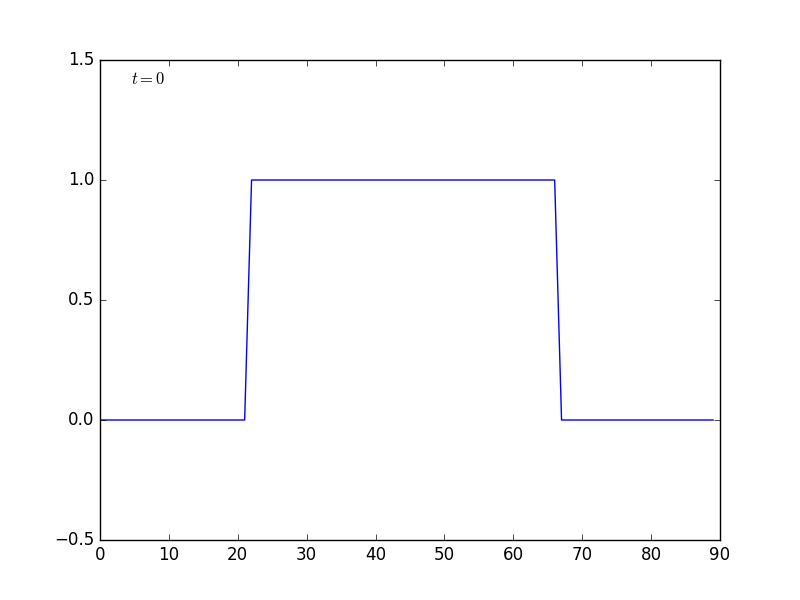
\includegraphics[scale=0.45]{CN_advection_frames/CN_advection_fig01.png}
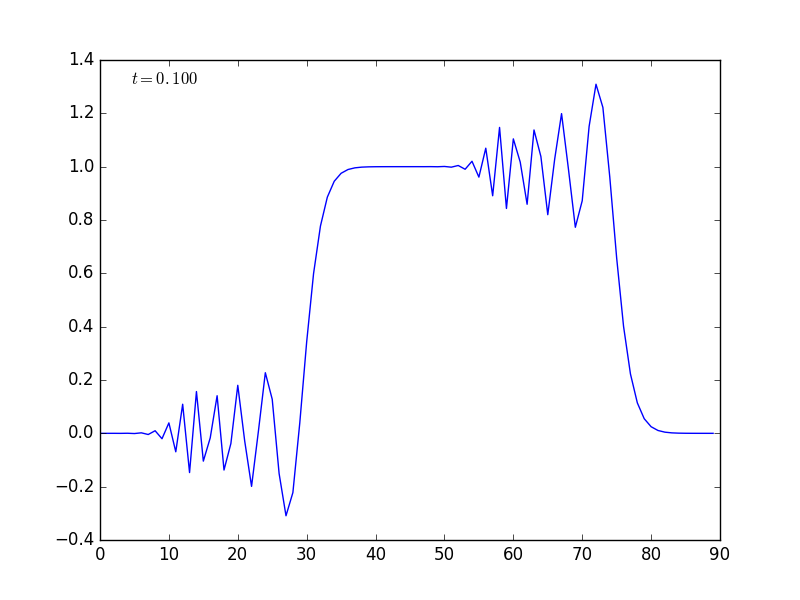
\includegraphics[scale=0.45]{CN_advection_frames/CN_advection_fig03.png}
\end{figure} 
\begin{figure}[H]
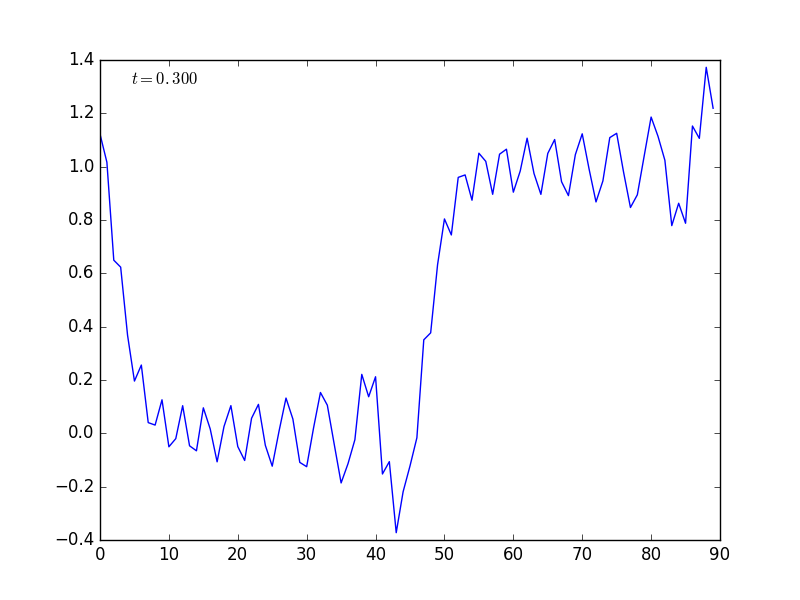
\includegraphics[scale=0.45]{CN_advection_frames/CN_advection_fig05.png}
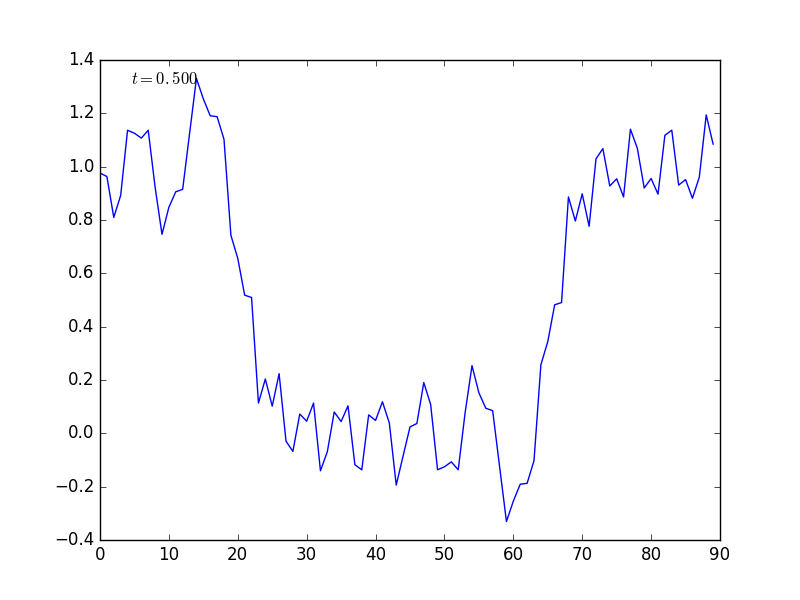
\includegraphics[scale=0.45]{CN_advection_frames/CN_advection_fig07.png}
\end{figure} 
\begin{figure}[H]
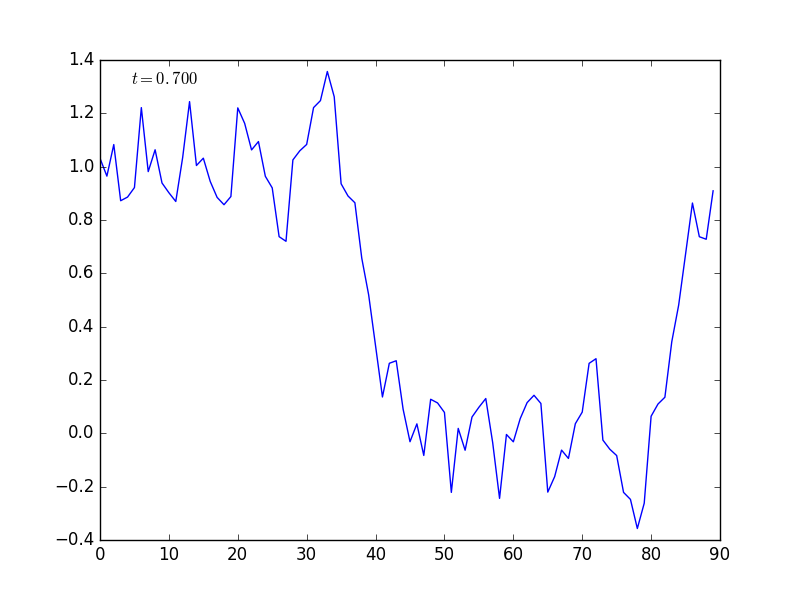
\includegraphics[scale=0.45]{CN_advection_frames/CN_advection_fig09.png}
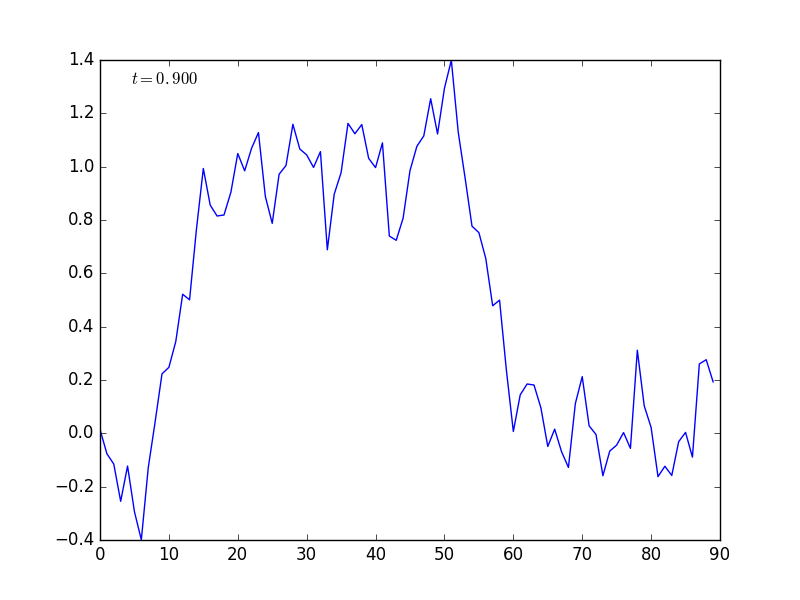
\includegraphics[scale=0.45]{CN_advection_frames/CN_advection_fig11.png}
\end{figure} 

\item Compute the relative phase error as arg($g(\theta)$)/($-\nu\theta$), where $g$ is the amplification factor and $\theta = \xi\Delta x$, and plot it for $\theta\in[0,\pi]$.  How does the relative phase error and lack of amplitude error relate to the numerical solutions you observed in part (b).
\end{enumerate}

The phase of $g$ is given by
$$\arg(g(\theta)) = \arctan\qty(\dfrac{\Im(g)}{\Re(g)})= \arctan\qty(\dfrac{-\nu\sin\theta}{1-\frac{\nu^2}{4}\sin^2\theta}) $$
In the limit of small $\theta$, we take the Taylor expansion of $\arctan$ about $\theta=0$:
$$\arg(g(\theta)) = \qty(\dfrac{-\nu\sin\theta}{1-\frac{\nu^2}{4}\sin^\theta}) - \qty(\dfrac{-\nu\sin\theta}{1-\frac{\nu^2}{4}\sin^\theta})^3/3 + h.o.t.$$
And then we use the expansions of $\sin\theta$ and $\frac{1}{1-x}$ about 0 together:
\begin{align*}
\arg(g(\theta)) &= -\nu\qty(\theta-\frac{\theta^3}{6}+\dots)\qty(1+\frac{\nu^2}{4}(\theta^2 + \dots)) - \qty(-\nu\qty(\theta-\frac{\theta^3}{6}+\dots)\qty(1+\frac{\nu^2}{4}(\theta^2 + \dots)))^3/3 \\
&= -\nu \theta + \frac{\nu\theta^3}{6} - \frac{\nu^3\theta^3}{4} + \dots + \dfrac{\nu^3\theta^3}{3} + \dots \\
&= -\nu \theta + \theta^3\qty(\frac{\nu}{6} - \frac{\nu^3}{4}+\dfrac{\nu^3}{3}) + h.o.t.
\end{align*}
Then the relative phase is 
$$\arg(g(\theta))/(-\nu\theta) = 1 - \theta^2\qty(\dfrac{2+\nu^3}{12}).$$
The following figure shows a plot of the relative phase for $\nu=0.9$, $\theta \in [0,\pi]$:
\begin{figure}[H]
\centering\begin{tikzpicture}
\begin{axis}[xmin=0,xmax=3.14, ylabel={Relative Phase}, xlabel={$\theta$}, xtick={0, 1.55, 3.14}, xticklabels={0, $\pi/2$, $\pi$}, ytick={1,0,-1}]
\addplot[domain=0:3.2, dashed] {0};
\addplot[domain=0:3.14] {1 - (x^2)*(2+0.9^3)/12};
%\addplot coordinates {(0,0) (10,22) (20,35) (30,42) (40,47) (50,50) (60,51)};
\end{axis} \end{tikzpicture}\end{figure}
What we see is that for the higher frequencies, ($\theta >\pi/2$), there is enormous relative phase lag, the highest frequencies being nearly lagging by nearly $200\%$.  The lack of amplitude error in conjunction with this phase lag causes the unphysical behavior we observed in the numerical solution in part b.  In contrast to Upwinding and Lax-Wendroff, in this scheme the amplitudes of the high frequencies aren't damped at all due to the non-dissipative nature of this scheme (as we showed in part a).  Then since the amplitudes are the high frequencies aren't damped, the enormous phase lag completely dominates the numerical solution, and the numerical solution quickly does not even resemble the real solution.

\end{document}